\documentclass{beamer}
\newcommand{\plt}{../../plots}
\usepackage{media9}
\addmediapath{\plt}

\mode<presentation> {

% The Beamer class comes with a number of default slide themes
% which change the colors and layouts of slides. Below this is a list
% of all the themes, uncomment each in turn to see what they look like.

%\usetheme{default}
%\usetheme{AnnArbor}
%\usetheme{Antibes}
%\usetheme{Bergen}
%\usetheme{Berkeley}
%\usetheme{Berlin}
%\usetheme{Boadilla}
\usetheme{CambridgeUS}
%\usetheme{Copenhagen}
%\usetheme{Darmstadt}
%\usetheme{Dresden}
%\usetheme{Frankfurt}
%\usetheme{Goettingen}
%\usetheme{Hannover}
%\usetheme{Ilmenau}
%\usetheme{JuanLesPins}
%\usetheme{Luebeck}
% \usetheme{Madrid}
%\usetheme{Malmoe}
%\usetheme{Marburg}
%\usetheme{Montpellier}
%\usetheme{PaloAlto}
%\usetheme{Pittsburgh}
%\usetheme{Rochester}
%\usetheme{Singapore}
%\usetheme{Szeged}
%\usetheme{Warsaw}

% As well as themes, the Beamer class has a number of color themes
% for any slide theme. Uncomment each of these in turn to see how it
% changes the colors of your current slide theme.

%\usecolortheme{albatross}
%\usecolortheme{beaver}
%\usecolortheme{beetle}
%\usecolortheme{crane}
%\usecolortheme{dolphin}
%\usecolortheme{dove}
%\usecolortheme{fly}
%\usecolortheme{lily}
%\usecolortheme{orchid}
%\usecolortheme{rose}
%\usecolortheme{seagull}
%\usecolortheme{seahorse}
%\usecolortheme{whale}
%\usecolortheme{wolverine}

%\setbeamertemplate{footline} % To remove the footer line in all slides uncomment this line
%\setbeamertemplate{footline}[page number] % To replace the footer line in all slides with a simple slide count uncomment this line

%\setbeamertemplate{navigation symbols}{} % To remove the navigation symbols from the bottom of all slides uncomment this line
}

\usepackage{graphicx} % Allows including images
\usepackage{booktabs} % Allows the use of \toprule, \midrule and \bottomrule in tables

%----------------------------------------------------------------------------------------
%   TITLE PAGE
%----------------------------------------------------------------------------------------
\setbeamertemplate{itemize items}[circle]
\setbeamertemplate{enumerate items}[circle]

\title[Motivic analysis]{Motivic analysis of neuronal signals} % The short title appears at the bottom of every slide, the full title is only on the title page

\author{Athul Vijayan} % Your name
\institute[DON Lab] % Your institution as it will appear on the bottom of every slide, may be shorthand to save space
{
IIT Madras \\ % Your institution for the title page
\medskip
\textit{athulvijayan6@gmail.com} % Your email address
}
\date{\today} % Date, can be changed to a custom date

\begin{document}

\begin{frame}
\titlepage % Print the title page as the first slide
\end{frame}

\begin{frame}
\frametitle{Overview}

\end{frame}

\begin{frame}
\frametitle{Experiment}
\begin{columns}[c] % The "c" option specifies centered vertical alignment while the "t" option is used for top vertical alignment

\column{.45\textwidth} % Left column and width
\textbf{Heading}

\column{.5\textwidth} % Right column and width
\end{columns}

\end{frame}

\begin{frame}
\frametitle{Experiment}
\begin{center}
\includemedia[
    activate=pageopen,
    width=0.75\textwidth
]{}{ani.mp4}
\end{center}
\end{frame}

\begin{frame}
\frametitle{Background}
\textbf{Orientation and Directional selectivity of neurons in V1}
\begin{itemize}
    \item Blah blah blah
    \item Blah blah blah
    \item Blah blah blah
    \item Blah blah blah
\end{itemize}
\begin{columns}[c]
\column{.45\textwidth} % Left column and width
\begin{figure}
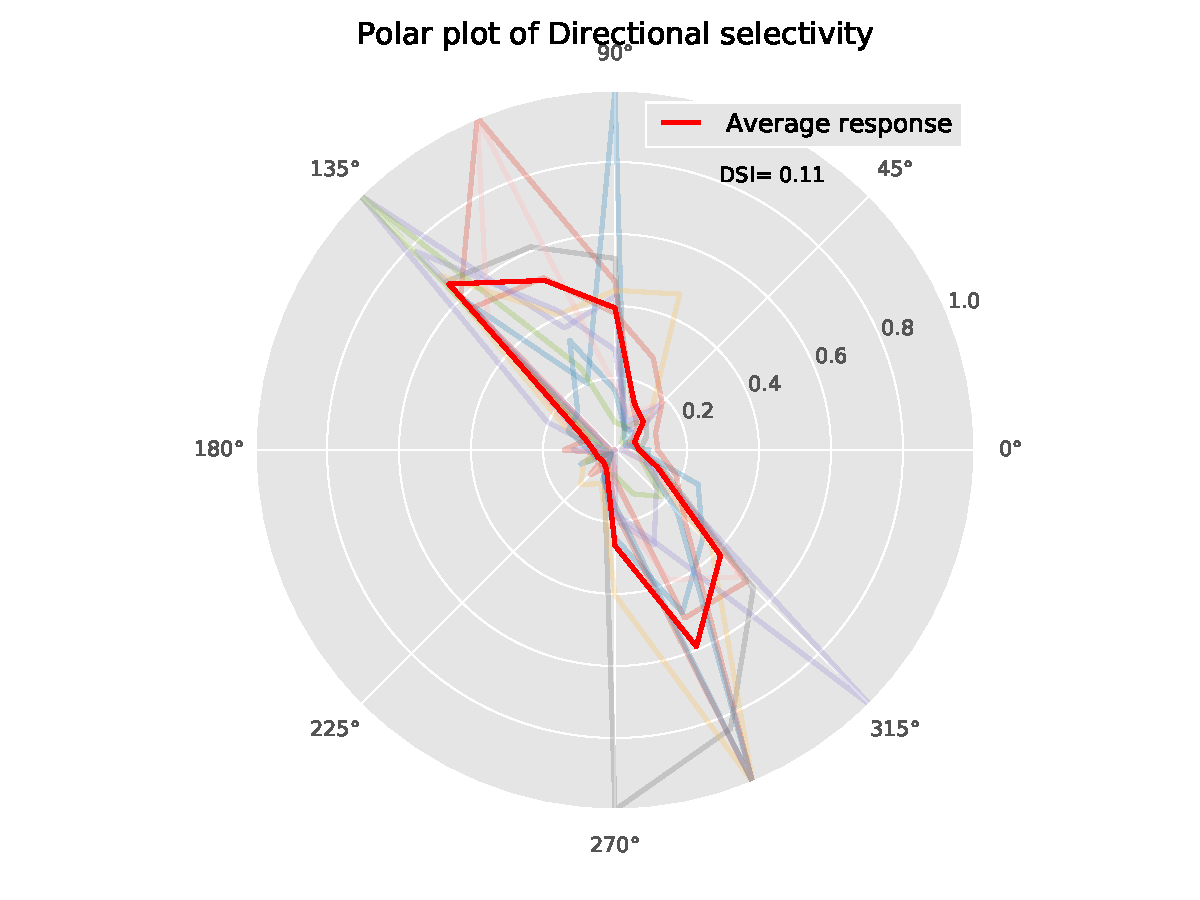
\includegraphics[width=0.8\linewidth]{\plt/gratings_dirpolar_2016_04_24_14_08_33.pdf}
\end{figure}
\column{.5\textwidth} % Right column and width
\begin{figure}
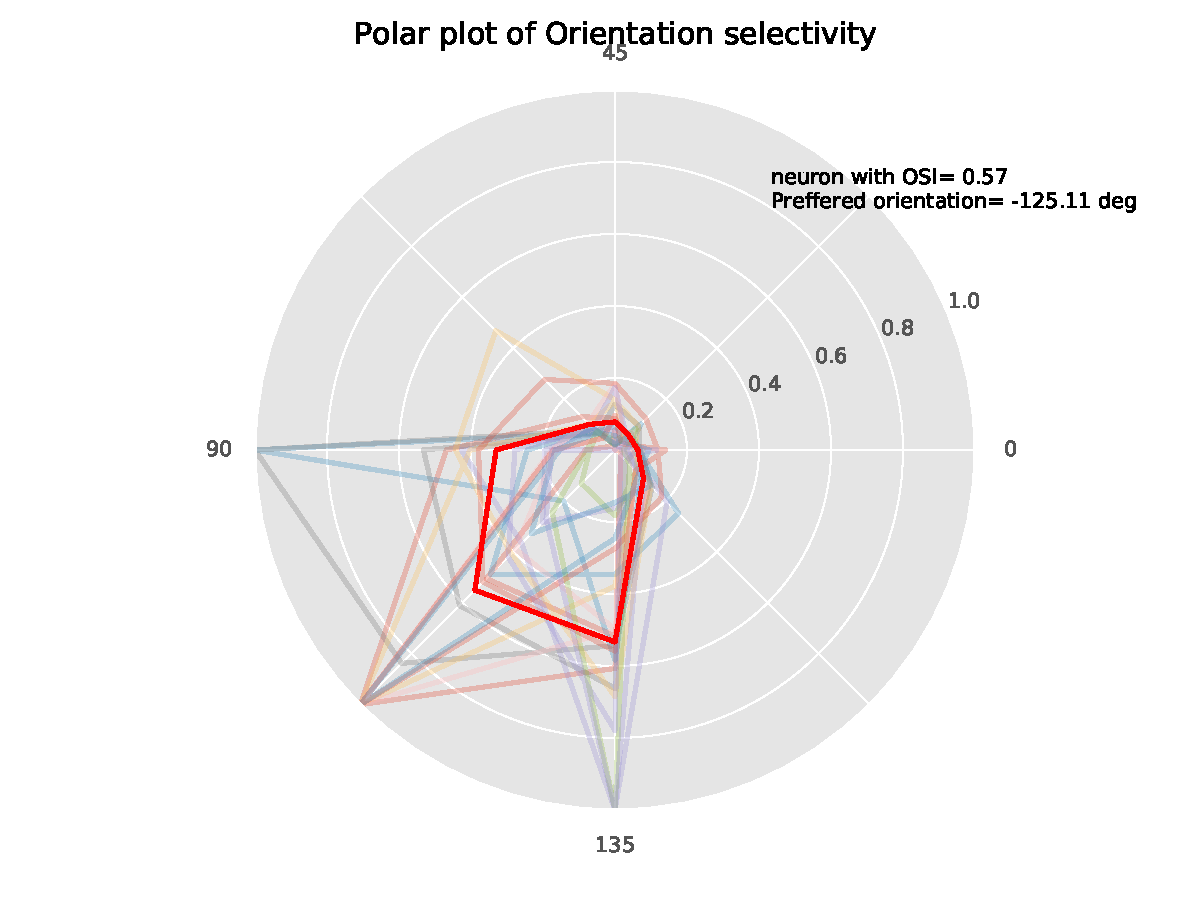
\includegraphics[width=0.8\linewidth]{\plt/gratings_oripolar_2016_04_24_14_08_33.pdf}
\end{figure}
\end{columns}
\end{frame}

\begin{frame}
\frametitle{Motivation}

\end{frame}

\begin{frame}
\frametitle{Reliability and correlation}
\begin{block}{Reliability Measure}
$$R_A = \frac{2}{T^2 - T}\sum_{i=1}^T \sum_{j=i+1}^T \rho(f_{i, A}, f_{j, A})$$
\end{block}
where $f_{i, A}$ is the response of neuron to $i^{th}$ trial of movie A and $\rho$ is the Pearson correlation.
\end{frame}

\begin{frame}
\frametitle{ACF analysis}

\end{frame}

\begin{frame}
\frametitle{ACFGram}
\begin{figure}
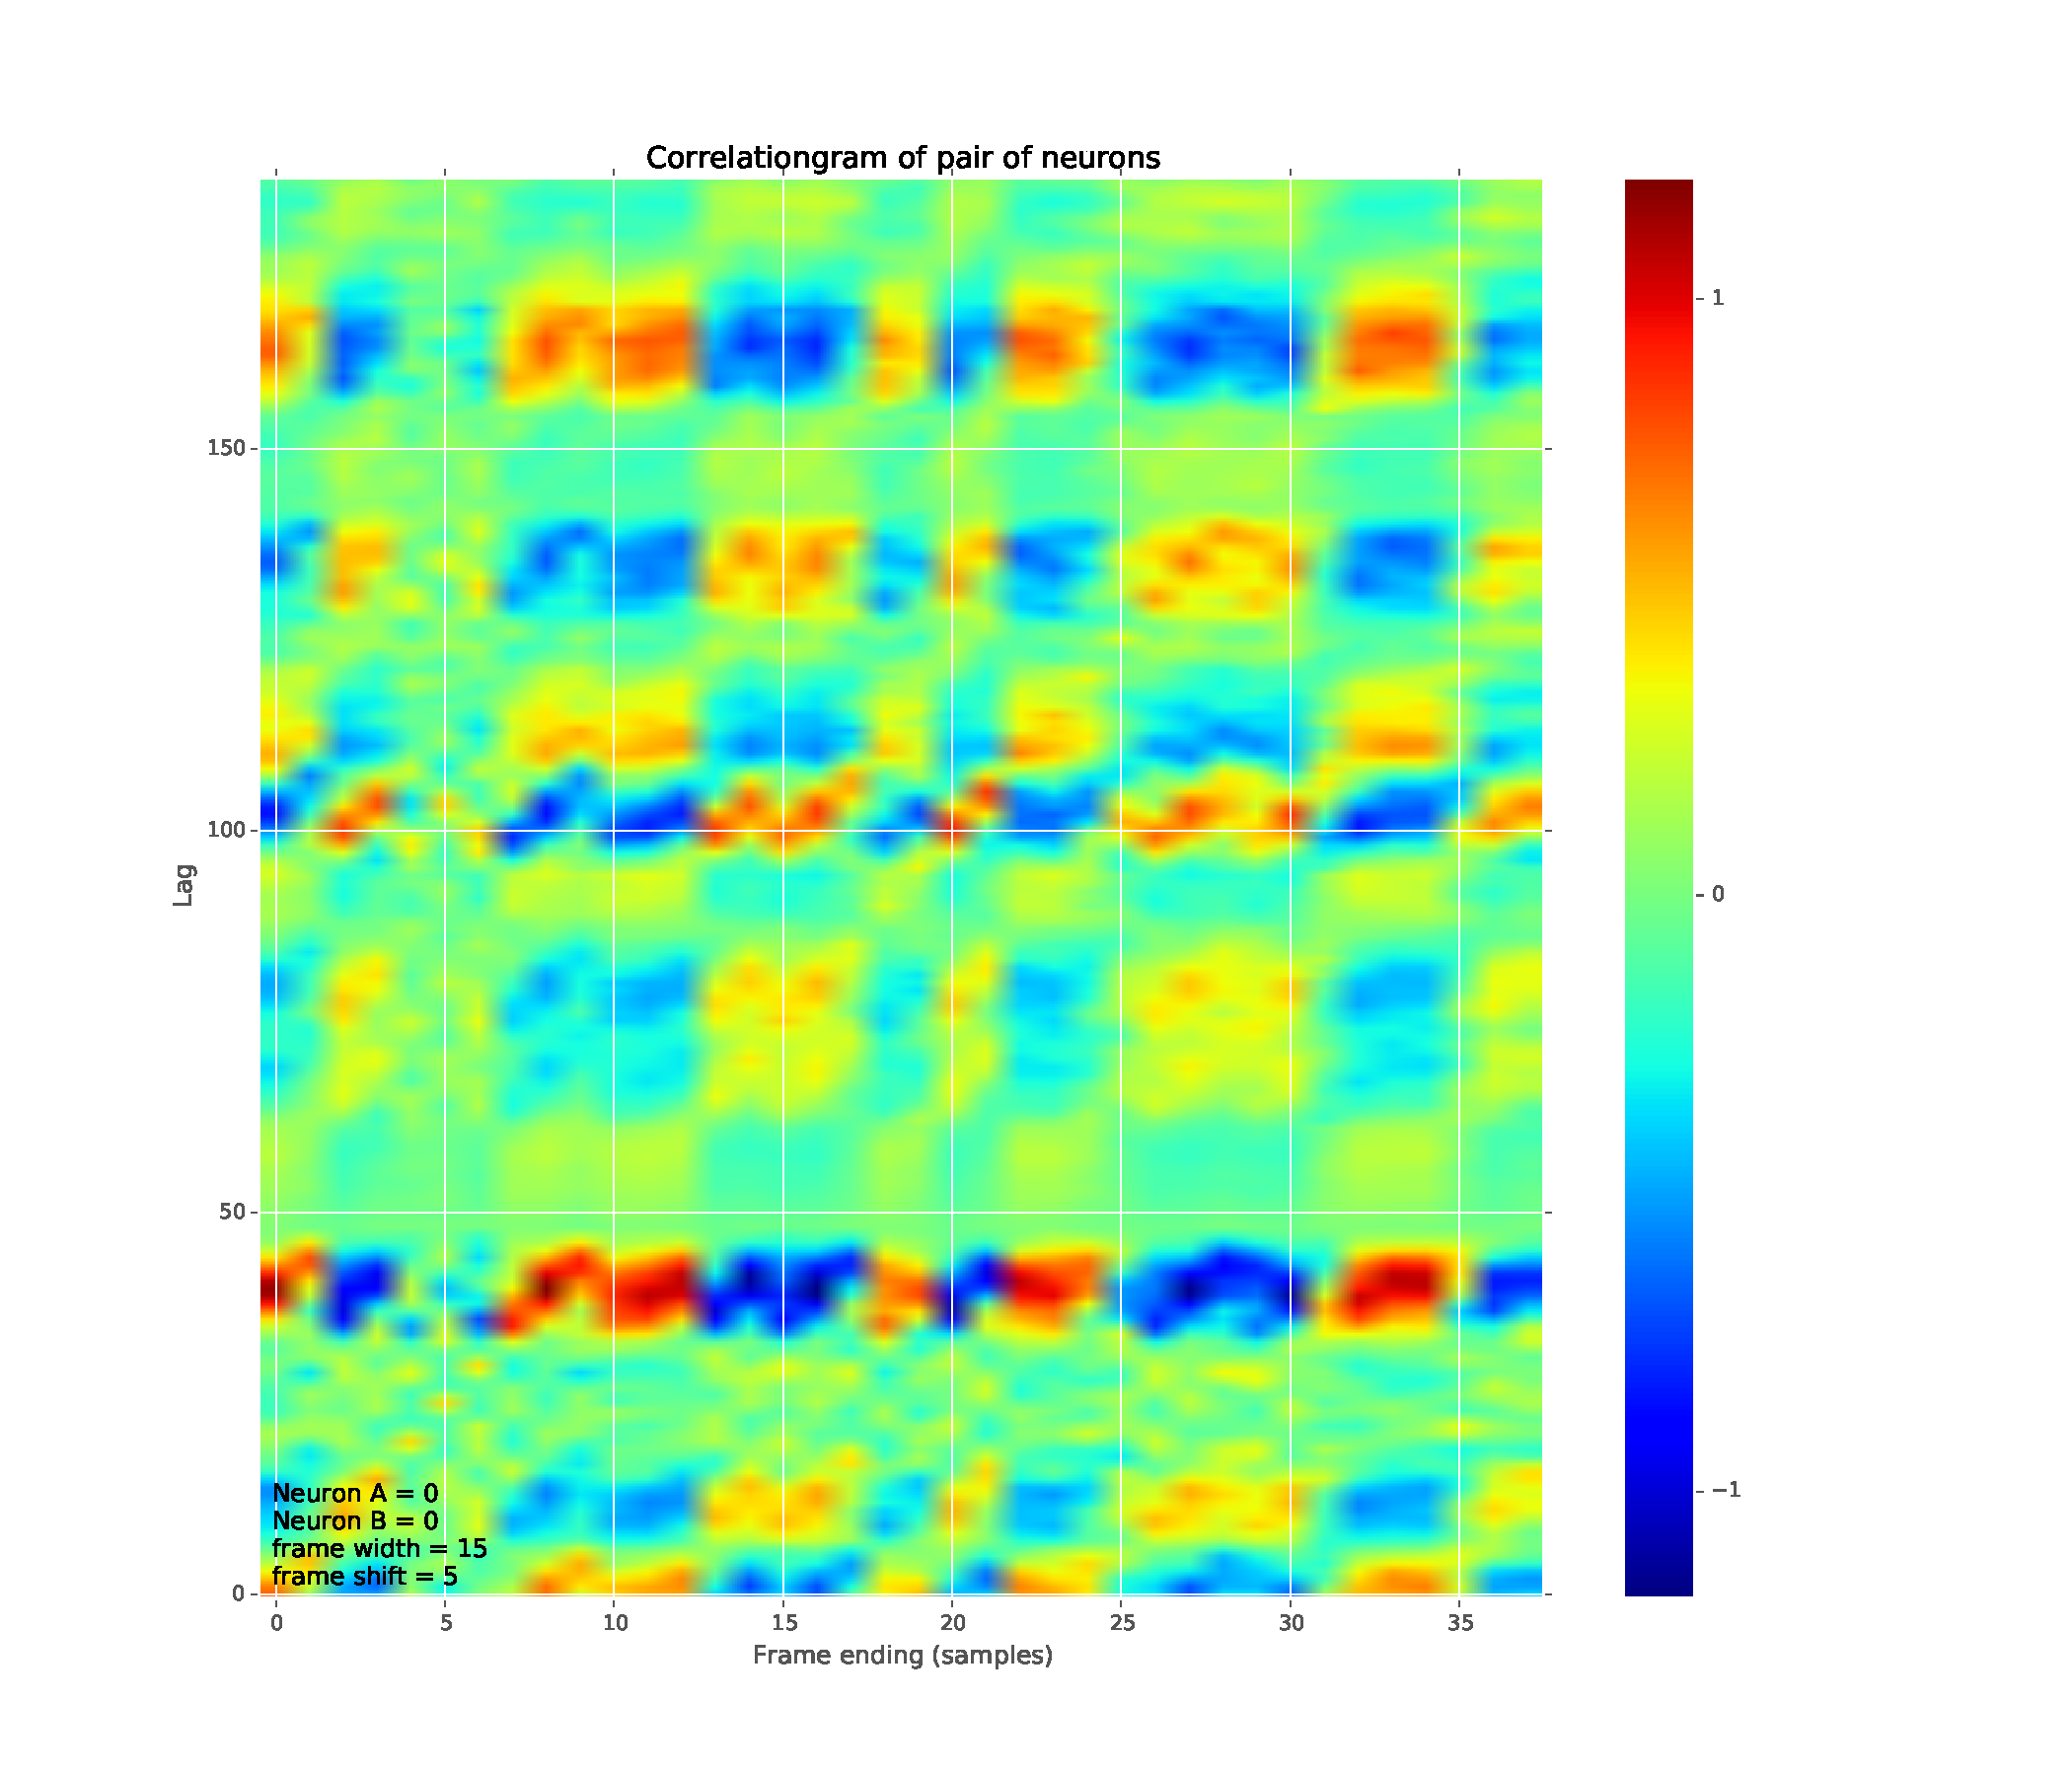
\includegraphics[width=0.8\linewidth]{\plt/acfMain_corrGram_2016_02_05_16_49_00.pdf}
\end{figure}
\end{frame}

\begin{frame}
\frametitle{Subsequence detection using RLCS}

\end{frame}

%------------------------------------------------
\begin{frame}
\frametitle{References}
\footnotesize{
\begin{thebibliography}{99} % Beamer does not support BibTeX so references must be inserted manually as below
\bibitem[Smith, 2012]{p1} John Smith (2012)
\newblock Title of the publication
\newblock \emph{Journal Name} 12(3), 45 -- 678.
\end{thebibliography}
}
\end{frame}
%----------------------------------------------------------------------------------------

\end{document} 